\documentclass[12pt]{article}
\usepackage{amsmath}
\usepackage[lmargin = 1in, rmargin = 1in, tmargin = 1in, bmargin = 1in]{geometry}
\usepackage[none]{hyphenat}
\usepackage{graphicx}
\usepackage{subcaption}
\usepackage{float}

\title{\textbf{Problem 1(2)\\Gradient Descent Implementation}}
\author{Aditya Vipradas\\ASU ID: 1209435588}
\begin{document}
\maketitle
The gradient descent method is implemented with the stopping criterion of 1e-6 and without the Armijo line search. The initial guess value is (1,1). The convergence and contour plots obtained are as follows. As observed, the values of $A_{12}$ and $A_{21}$ are 1.9572 and 1.685 respectively which agree with the values obtained by the implementation of the lsqnonlin command in MATLAB. See the attached gradient descent codes.
\begin{figure}[H]
\begin{center}
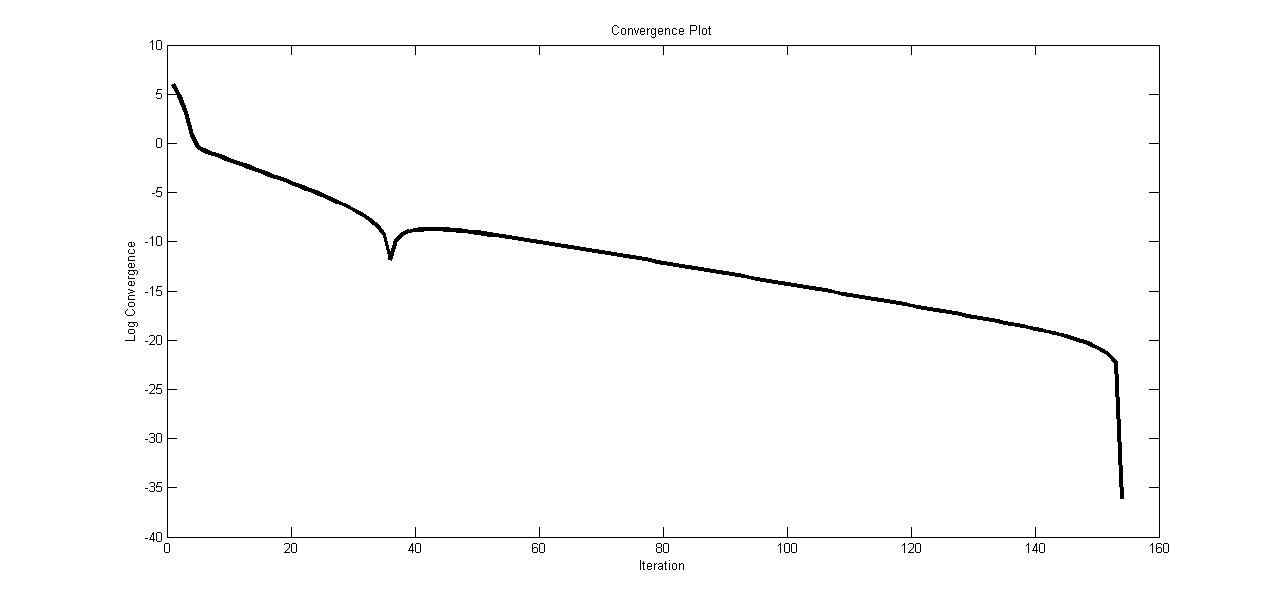
\includegraphics[scale=0.4]{convergence.jpg}
\caption{Convergence plot}  
\end{center}
\end{figure}
\begin{figure}[H]
\begin{center}
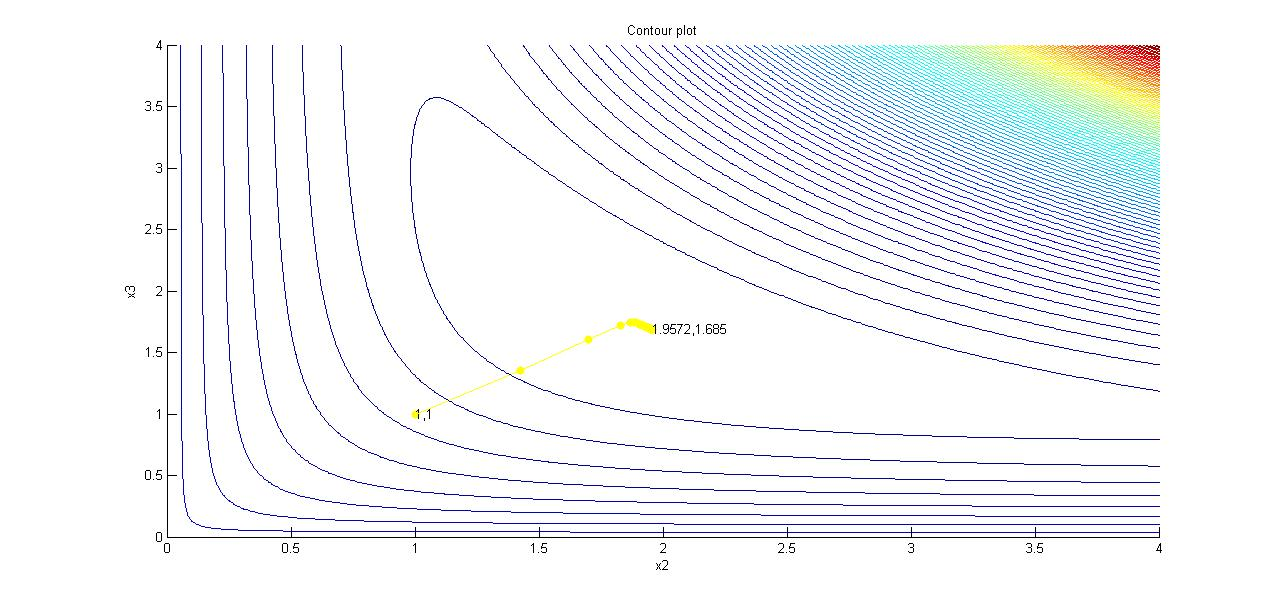
\includegraphics[scale=0.4]{contour.jpg}
\caption{Contour plot with the values of $A_{12}$ and $A_{21}$}  
\end{center}
\end{figure}
\end{document}